\documentclass{standalone}
\usepackage{tikz}
\usepackage{ctex,siunitx}
\setCJKmainfont{Noto Serif CJK SC}
\usepackage{tkz-euclide}
\usepackage{amsmath}
\usetikzlibrary{patterns, calc,3d}
\usetikzlibrary {decorations.pathmorphing,decorations.pathreplacing,decorations.shapes}
\begin{document}
\small
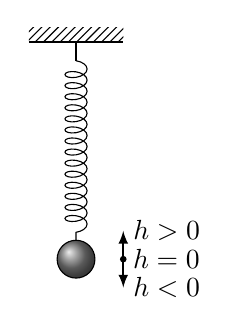
\begin{tikzpicture}[>=latex,scale=1.2]
  \fill[pattern=north east lines](-0.5,0)rectangle(0.5,0.15);
  \draw[thick](-0.5,0)--(0.5,0);
  \draw(0,0)--(0,-0.2);
  \draw[decorate,decoration={coil,segment length=4pt,amplitude=4pt}](0,-0.2)--(0,-2.1);
  \draw[ball color=gray](0,-2.3)circle(0.2);
  \draw[semithick,<->](0.5,-2.6)node[right]{$h<0$}--(0.5,-2.0)node[right]{$h>0$};
  \fill(0.5,-2.3)circle(1pt)node[right]{$h=0$};
\end{tikzpicture}
\end{document}